% Section 1. Rewritten 2026-10-06 (loop0009 item 02) after
% paper1/review_readability.md section 7 and the owner's notes in
% Ralph_Loops/loop0009/TASK.md. The history paragraph keeps the owner's account
% of how the thesis's Table 2.1 was assembled (first version written the same
% day from literature/linhares_2001_phd_thesis_industrial_pattern_sequencing.pdf).
% Figure 1.1: python -m paper1.intro_figure (numbers checked by
% tests/test_intro_figure.py). Counts of rows: Table 2.1 (tab:master).
% Headline numbers: Sections 3-5 and their sources there.
\section{Introduction}
\label{sec:intro}

A factory makes a set of patterns, one at a time, and each customer's order
needs some of them. A customer's stack opens when the first pattern the
customer needs is made, and it closes when the last one is made. The
\emph{minimization of open stacks problem} (MOSP) asks for the order of the
patterns that keeps the fewest stacks open at any one time. In the cutting
industry, where the problem arose, the patterns are cutting patterns and the
customers are piece types \citep{Yanasse1997b}. Figure~\ref{fig:example}(a)
gives a small instance. Six customers, $a$ to $f$, need four patterns:
$P_1=\{a,b\}$, $P_2=\{b,c,d\}$, $P_3=\{c,d,e\}$ and $P_4=\{e,f\}$. Made in
order A, $P_1P_2P_3P_4$, the patterns keep at most 3 stacks open. Made in order
B, $P_1P_3P_4P_2$, they keep 5 open, because customer $b$ is served first but
waits for $P_2$, which comes last. Of the 24 orders, 2 reach 3 (order A and its
reverse), 16 give 4 and 6 give 5.

\begin{figure}[tbp]
\centering
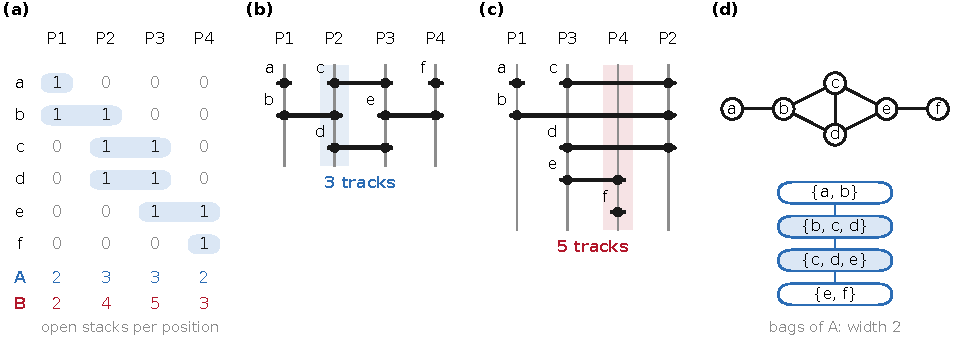
\includegraphics[width=\linewidth]{sec1_fig1_example.pdf}
\caption{One instance, three readings, one number. (a) Six customers and four
patterns, with each customer's open stack shaded in order A; order A keeps at
most 3 stacks open and order B at most 5, and only 2 of the 24 orders reach 3.
(b, c) The same matrix as a gate matrix layout: the same two orders need 3 and
5 tracks (the shaded gate is where the density peaks). (d) The same matrix as a
\emph{graph}, one clique per pattern: the open sets of order A are the bags of a path
decomposition of width 2, so the optimum is the pathwidth plus one
(Theorem~\ref{thm:mosp}).}
\label{fig:example}
\end{figure}

The same matrix is a problem in VLSI design. In a \emph{gate matrix layout}
the patterns are gates, drawn as vertical lines in some order, and the
customers are nets. Each net is a horizontal wire from the first gate it
connects to the last, and wires that overlap must lie on different horizontal
tracks. The task is to order the gates so that the fewest tracks suffice.
Figure~\ref{fig:example}(b) and (c) draw the two orders. The wires are the same;
only the gate order changes which wires overlap. Order A packs into 3 tracks
and order B needs 5. The number of tracks a gate order needs is its
\emph{density}, the most wires crossing any one gate, and that is exactly the
number of open stacks there. So the two problems compute the same number from
the same matrix \citep[Proposition~2]{LY2002}.

The same matrix is also a graph. Make each customer a vertex, and join two
customers when some pattern needs both, so that each pattern becomes a clique
(Figure~\ref{fig:example}(d)). Write down, for order A, the set of open stacks
at each position: $\{a,b\}$, $\{b,c,d\}$, $\{c,d,e\}$, $\{e,f\}$. These sets
cover every vertex and every edge, and each customer appears in a run of
consecutive sets. In graph theory such a sequence is a \emph{path
decomposition}, its sets are \emph{bags}, and its width is the size of its
largest bag minus one. The least width over all path decompositions is the
\emph{pathwidth} of the graph, here 2. The construction works in both
directions, so the fewest open stacks is always the pathwidth plus one
(Theorem~\ref{thm:mosp}).

The same graph is, finally, a sparse symmetric matrix of numerical linear
algebra, with a nonzero wherever two customers share a pattern. The frontal
method eliminates its rows one at a time and must keep in memory the
\emph{wavefront}, the rows already touched but not yet eliminated. Eliminating
the customers in the order $a,b,\dots,f$ keeps at most 3 rows active at once,
and no order does better: the least maximum wavefront is again the pathwidth
plus one (Theorem~\ref{thm:core}). This fourth reading is not in our 2002
table, and we add it below.

\begin{table}[tbp]
\centering
\caption{Twelve problems from three fields, published as one family: eight
rows are exact, counting the pathwidth row itself; two are bands; two are false
as the table states them. Our own table of 2002, reproduced from
\citet[Table~1, p.~1764]{LY2002} with its row order, wording and references as
printed, and its caption: ``Display of a family of equivalent problems studied
independently on the literature''. The shaded column corrects it: it gives the
relation to pathwidth ($\pw$) that is true, proved in Section~\ref{sec:equiv}
(Table~\ref{tab:master}). The last three rows, below the rule, are new:
members of the family that the table missed, which bring a fourth field,
numerical linear algebra.}
\label{tab:ly2002}
\small
\setlength{\tabcolsep}{3.5pt}
\begin{tabular}{@{}lll>{\columncolor{black!7}}l@{}}
\toprule
Problem & Discipline & References & This paper \\
\midrule
MOSP & Operations research & \citet{Yanasse1997b}; \citet{LY2002ref4} & exact: $\pw+1$ \\
Gate matrix layout & VLSI design & \citet{LY2002ref6}; \citet{LY2002ref8} & exact: $\pw+1$ \\
One-dimensional logic & VLSI design & \citet{LY2002ref7} & exact: $\pw+1$ \\
PLA folding & VLSI design & \citet{LY2002ref6} & false$^{a}$ \\
Interval thickness & Graph theory & \citet{LY2002ref5} & exact: $\pw+1$ \\
Node search game & Graph theory & \citet{LY2002ref9} & exact: $\pw+1$ \\
Edge search game & Graph theory & \citet{LY2002ref10} & band: $\pw$ to $\pw+2$ \\
Narrowness & Graph theory & \citet{LY2002ref11} & exact: $\pw+1$ \\
Split bandwidth & Graph theory & \citet{LY2002ref12} & band: $\pw$ to $\pw+1$ \\
Graph path-width & Graph theory & \citet{LY2002ref13} & exact: $\pw$ (reference) \\
Edge separation & Graph theory & \citet{LY2002ref14} & false$^{b}$ \\
Vertex separation & Graph theory & \citet{LY2002ref13} & exact: $\pw$ \\
\midrule
\emph{Progressive pebbling}$^{c}$ & Graph theory & \citet{LY2002ref10} & exact: $\pw+1$ \\
\emph{Vertex search}$^{d}$ & Graph theory & \citet{BRST1991} & exact: $\pw+1$ \\
\emph{Maximum wavefront}$^{e}$ & \begin{tabular}[t]{@{}l@{}}Numerical\\linear algebra\end{tabular} & \citet{KumfertPothen1997} & exact: $\pw+1$ \\
\multicolumn{4}{@{}l@{}}{\footnotesize\emph{New: not in \citet{LY2002}.}} \\
\bottomrule
\multicolumn{4}{@{}p{\linewidth}@{}}{\footnotesize $^{a}$Exact ($\pw+1$) for
multiple folding, with any number of nets per track.
$^{b}$As cutwidth; the vertex separator game of the same reference is exact
($\pw$, for graphs with an edge).
$^{c}$Added by us. Its relation to pathwidth is proved in two papers the table
already cites, for other rows: \citet[Thms~2--3]{LY2002ref14} and
\citet[Thm~3.1]{LY2002ref10}. We prove it in Lean (Appendix~\ref{app:thirteenth}).
$^{d}$Added by us. Searchers occupy vertices and an invisible fugitive moves
along unguarded paths. Exact on every graph with a vertex, edgeless ones
included \citep[(5.1)]{BRST1991}, and equal to node search when the graph has
an edge. We prove it in Lean, following their construction for the upper bound
(Appendix~\ref{app:thirteenth}).
$^{e}$Added by us. The least, over symmetric orderings of a sparse symmetric
matrix with nonzero diagonal, of the largest wavefront
\citep[\S2.1]{KumfertPothen1997}; it is narrowness in another form. The source
defines it but does not state the equality, which we prove in Lean
(Appendix~\ref{app:thirteenth}).}
\end{tabular}
\end{table}

We collected twelve such problems \citep{LY2002}, from operations research,
VLSI design and graph theory, in the table that Table~\ref{tab:ly2002}
reproduces. Each computes, on corresponding inputs, ``a function $f(\Pi)$ that
is either equal to the number of open stacks or closely related to it (plus or
minus one)'' \citep[p.~1764]{LY2002}. The table gives a reference for each
problem, but no proofs and no graph of which problem reduces to which. ``Plus
or minus one'' has two readings. Under the \emph{literal} reading, $f$ is
within one of the number of open stacks on every input. Under the
\emph{fixed-offset} reading, $f$ equals the number of open stacks plus one
constant, the same on every input. Only the second makes solving one problem
the same as solving another. We call the problems that are, on every input,
pathwidth or pathwidth plus one the \emph{pathwidth complex}: most of the
table, and three problems we originally missed. Pathwidth is the quantity
through which every true relation in the table is proved
(Section~\ref{sec:equiv}). It is also the name the literature uses, more than
three times as often as the other eleven names combined (Section~\ref{sec:names}),
so a reader who searches under ``open stacks'' or ``gate matrix layout''
misses most of what is known. The communities that could have checked the
table rarely read each other: of 844 works that cite the table's papers, only
six cite both an open-stacks paper and a graph-theory paper.

The table is ours, and its history explains why no one checked which of its
equalities are true. It was first printed in 2001, in the first author's
doctoral thesis \citep[Table~2.1, p.~13]{Linhares2001}, supervised by the
second author, which proved MOSP NP-hard and equal to gate matrix layout. Its
rows were collected over the years of the doctorate, while reading the
literature of each field. Each came with a reference and nothing else: no
row's relation to open stacks was checked, and no published proof was
restated. The table appeared again, row for row, as Table~1 of \citet{LY2002},
and it has been read since as a statement of equivalence.
\citet{GarciaDeLaBandaStuckey2007}, for instance, credit the speed of their
search in this journal to ``the fact that the problem is fixed parameter
tractable (Linhares and Yanasse 2002)''. When MOSP was set as the first
Constraint Modelling Challenge in 2005, the organisers' report pointed to the
table for the problems equivalent to it, ``including graph path-width'', and
credited the second author with the idea of permuting customers rather than
products \citep{SmithGent2005,Yanasse1997b}, the idea on which Chu and
Stuckey's customer search (Section~\ref{sec:search}) branches. So the table is
already used to justify algorithms, and whether it is true matters. If it is
true, \emph{every result} about any one of the twelve problems transfers to
\emph{all} the others. Looking back, the table was the thesis's most important
finding, and this article does what the thesis did not: it states each problem
precisely, proves what is true and refutes what is not. This paper asks:
\emph{which of the equalities in the Linhares--Yanasse table are true, and what
follows when results, algorithms and benchmarks are moved between the twelve
problems through pathwidth?}

\paragraph{Three more members.} The table was also incomplete. Progressive
pebbling, a game in which pebbles are placed on the vertices of a graph and
each vertex is pebbled once, needs exactly pathwidth plus one pebbles
\citep[Thm~3.1]{LY2002ref10}, and Lengauer's black-white pebbling of a
directed acyclic graph equals the pathwidth of its undirected version plus one
\citep[Thm~2]{LY2002ref14}. Both theorems are in papers that the table
already cites, for its edge-search and edge-separation rows, yet pebbling
itself is not among its problems. \citet[(5.1)]{BRST1991} search for a fugitive
who hides in the vertices, not the edges, and need exactly pathwidth plus one
searchers on every graph with a vertex, including the edgeless graphs where the
table's node search row fails. From numerical linear algebra, the wavefront of
the frontal method, met above \citep[\S2.1]{KumfertPothen1997}, is the problem
of the table: the least maximum wavefront is the pathwidth of the matrix's
graph plus one, on every nonempty matrix. We add the three as the last rows of
Table~\ref{tab:ly2002}, marked as new, and prove all three relations in the
Lean proof assistant (Appendix~\ref{app:thirteenth}). For pebbling and the
vertex search, what is new is the membership: the equivalences were published,
but the table did not include them. For the wavefront the equality itself is
ours: it is elementary, as the wavefront is narrowness read in another form,
but no source we have read states it.

\paragraph{What we find.}
\begin{itemize}
\item \emph{The table, settled.} Eight of the twelve rows are exact: on every
  input, outside degenerate cases such as an empty graph, the problem equals
  pathwidth or pathwidth plus one (the pathwidth row itself is one of the
  eight). Two rows, split bandwidth and edge
  search, lie in \emph{bands}: within one and two of pathwidth, but not at a
  fixed offset. Two rows, PLA folding and edge
  separation, are false as stated, with counterexamples. A variant of each
  false row is exact. Three problems outside the table are exact members
  too: progressive pebbling, a vertex search, and the maximum wavefront of
  sparse matrix elimination (Section~\ref{sec:equiv}).
\item \emph{One name.} The literature has settled on ``pathwidth'', which has
  more than three times as many relevant works as the other eleven names
  combined. Since 2005, after pathwidth, the most active name of the twelve is
  MOSP, and the best exact search for the whole family came from that
  community, by way of the 2005 Constraint Modelling Challenge
  (Section~\ref{sec:names}).
\item \emph{Two false theorems, and our correction.} The best exact algorithm
  for MOSP, the \emph{customer search} of \citet{ChuStuckey2009}, which we call
  the previous algorithm, branches on the order in which customers' stacks
  close, and it is also a pathwidth algorithm. We prove in Lean, however, that
  two of its published dominance theorems, the \emph{definite move} and the
  \emph{better move}, are false, as are their later restatements
  \citep{Chu2011,Fink2012}: each can discard the last remaining solution at a
  node of the search tree. We provide a counterexample instance: our
  implementation of their algorithm, with its better move off, obtains an
  optimum of 7, while our corrected version obtains 6, provable also by a SAT
  (Boolean satisfiability) solver. This is a theorem checked in Lean: the
  whole run of their algorithm on the instance, and its optimum of 6
  (Theorem~\ref{thm:wrong}). Our corrected
  definite move was also found by Tamaki as a lemma
  \citep[Lemma~1]{Kitsunai2016}, in the exact pathwidth literature; we show
  that it can be tested by one bipartite matching per candidate, and prove our
  corrected search sound. Our correction costs at most 2\% more search nodes
  on each group of benchmarks we measured.
\item \emph{A pathwidth solver.} Ported to graphs, our corrected search is an
  exact pathwidth solver, which we release. Within 600 seconds per graph it
  proves the pathwidth of 11,194 of the 11,534 Rome graphs, a graph-drawing
  benchmark of 10 to 110 vertices; all 50 trees of VSPLIB, a benchmark library
  for vertex separation; and 39 of its 73 Harwell--Boeing graphs, the sparsity
  patterns of engineering matrices. On each set this is as many graphs or more
  than the published branch and bound of \citet{CoudertMazauricNisse2016}
  (Section~\ref{sec:results}).
\item \emph{Benchmarks re-certified, and a dataset.} Our corrected search
  re-proved all 115 benchmark optima, on 113 distinct graphs, that rested on
  the previous algorithm, and none changed. We release 17,714 graphs, distinct
  up to isomorphism, from twenty benchmark collections of MOSP, VLSI layout,
  vertex separation, graph drawing and treewidth; 16,088 have a certified
  pathwidth with a layout that attains it, and so a certified value for every
  problem of the pathwidth complex (Section~\ref{sec:results}).
\end{itemize}

\paragraph{How to read the paper.} Section~\ref{sec:equiv} states the twelve
problems and proves what is true. Section~\ref{sec:names} measures which names
and communities the literature uses. Section~\ref{sec:search} reads the exact
open-stacks search as a pathwidth algorithm, finds the two false rules and
proves our corrected search sound. Section~\ref{sec:results} reports what our
corrected search costs, how it performs as a pathwidth solver, and the dataset, and Section~\ref{sec:closing} returns to the question this paper asks.
Every theorem we state is machine-checked in the Lean~4 proof assistant, unless
the text says otherwise. The
reader need not read Lean: each proof is given or cited in the text, and
Appendix~\ref{app:lean} maps each result to its formal statement.
Appendix~\ref{app:machinery-all} holds the supporting material,
and Appendix~\ref{app:names} the bibliometric method. The Lean development,
both solvers, the dataset and an independent checker for each are openly
available, the code and proofs as open source under the MIT licence
(page~\pageref{sec:data}).
